\section{Quotient circuits}
\label{sec:quotient}

In this section, we consider the cases where  $\mathcal{I}$
is the input for all the nodes within a same fiber, such that 
the fibration symmetry is preserved by the input. In this case, 
we can simplify the network representation by colapsing nodes 
belonging to the same fiber into one single node. This simplified
representation is referred as {\it quotient} or {\it base} network 
\cite{martin_ian_groupoids2006,Boldi2002,morone2020}. By performing this 
transformation, we observe that the possible paths from input to
the output of the network are also reduced, specially when we 
consider the fundamental fibration building blocks. The circuits 
considered here are defined as follows: given a fiber circuit
defined either by $n$ and $\ell$ for integer branching ratios or 
by $\phi_d$ and $\ell$ for golden ratios of fibonacci circuits, we 
add an extra node that is going to be regulated by all nodes 
withing the same fiber. The protein concentration of this external
gene is going to be defined as the input-output map, i.e., the 
output node of the network. Moreover, the input $\mathcal{I}$ 
regulates all nodes of the fiber. Thus, we reduce the circuit to 
its quotient form and analyze the nonlinear dynamics of this 
reduced input-output circuit according to the methods described in 
the previous sections.

\subsection{$|n = 1, \ell \rangle$ input-output circuit}

Here, we consider the fiber circuit defined by $n = 1$, called 
as Feed-Forward Fiber (FFF)\cite{transistor2019}. Depending 
on the type of internal regulation of the fiber, we denote this 
circuit either as SAT-FFF (for positive regulations) or UNSAT-FFF
(negative regulations). Considering the mRNA/Protein gene 
expression model (to describe in another section before), we have
that the input-output network and its quotient form is shown in 
Fig.~\ref{fig:n1_quot}.

\begin{figure}[H]
    \centering
    
\includegraphics[scale=0.5]{figs/quotient_n1.png}
    \caption{}
    \label{fig:n1_quot}
\end{figure}

\subsubsection{Admissible vector fields}

The general possible dynamics restricted by
the topology of this network is given by the following system of 
admissible equations \cite{martin_ian_groupoids2006}:
\begin{equation}
    \begin{aligned}
        \dot{x_1}^R &= f_{x_1^R}(x_1^R, \mathcal{I})\\
        \dot{x_1}^P &= f_{x_1^P}(x_1^P, x_1^R)\\
        \dot{x_2}^R &= f_{x_2^R}(x_2^R, x_1^P)\\
        \dot{x_2}^P &= f_{x_2^P}(x_2^P, x_2^R)\\
    \end{aligned},
\end{equation} 
where $\vec{F} = (f_{x_1^R}, f_{x_1^P}, f_{x_2^R}, f_{x_2^P})$ is 
the vector of nonlinear functions as described in 
section~\ref{sec:intro}. The Jacobian of this system is 
\begin{equation}
    J = 
    \begin{pmatrix}
        f_{x_1^R,x_1^R} & f_{x_1^R, x_1^P} & 0 & 0 \\
        f_{x_1^P,x_1^R} & f_{x_1^P,x_1^P} & 0 & 0 \\
        0 & f_{x_2^R,x_1^P} & f_{x_2^R,x_2^R} & 0 \\
        0 & 0 & f_{x_2^P,x_2^R} & f_{x_2^P,x_2^P} \\
    \end{pmatrix},
\end{equation} 
where we require that $f_{x_1^R, x_1^R} < 0$, $f_{x_1^P, x_1^P} < 0$, 
$f_{x_2^R, x_2^R} < 0$ and $f_{x_2^P, x_2^P} < 0$ to permit a 
stable equilibrium at $\vec{x_0}$. Moreover, the homeostasis matrix
is given by
\begin{equation}
    H = 
    \begin{pmatrix}
        f_{x_1^P,x_1^R} & f_{x_1^P,x_1^P} & 0 \\
        0 & f_{x_2^R,x_1^P} & f_{x_2^R,x_2^R} \\
        0 & 0 & f_{x_2^P,x_2^R} \\
    \end{pmatrix}.
\end{equation} 

\subsubsection{Combinations}

Considering the $| n=1, \ell \rangle$ fiber circuits observed in 
the \textit{E. Coli} genetic regulatory network, we have two 
possibilities, as mentioned before: the SAT-FFF and the UNSAT-FFF,
where here we do not take into account the regulators of the fiber
defined by $\ell$, since here their only purpose is to maintain 
the fibration symmetry of the network. For each one of the two 
possibilities there are 6 possibles combinations: two with equal 
external regulations to the output node (Fig.~\ref{(a,b,...)}), 
and one for the case where the types of regulations are 
alternated (Fig.~\ref{c,d,...}).  

\subsubsection{Special equations}

Now, considering the special equations as described in 
section.~\ref{sec:askds}, we have the following core 
differential equations for all SAT-FFF and UNSAT-FFF:

{
    \setlength{\tabcolsep}{10pt}
    \renewcommand{\arraystretch}{3.0}
\begin{table}[H]
    \centering
    \vspace{0.2cm}
    \begin{tabular}{|c|c|}
        \hline
        \textbf{SAT-FFF} & \textbf{UNSAT-FFF} \\
        \hline
        $\begin{aligned}
            \dot{x_1}^R &= -\delta_1 x_1^R + \gamma_1(1-S(x_1^P)) + I\\
            \dot{x_1}^P &= -\alpha_1 x_1^P + \beta_1 x_1^R
        \end{aligned}$ & 
        $\begin{aligned}
            \dot{x_1}^R &= -\delta_1 x_1^R + \gamma_1 S(x_1^P) + I\\
            \dot{x_1}^P &= -\alpha_1 x_1^P + \beta_1 x_1^R
        \end{aligned}$ \\[0.25cm]
        \hline

    \end{tabular}
\end{table}
}

Therefore, we can list all combinations for the external regulated
nodes $x_2^R$ and $x_2^P$ as 

{
\setlength{\tabcolsep}{10pt}
\renewcommand{\arraystretch}{3.0}
\begin{table}[H]
    \centering
    \vspace{0.2cm}
    \hspace*{-1cm}
    \begin{tabular}{|c|c|c|}
        \hline
         & \textbf{SAT-FFF} & \textbf{UNSAT-FFF} \\
        \hline
        (a) & $\begin{aligned}
            \dot{x_2}^R &= -\delta_2 x_2^R + \gamma_2(1-S(x_1^P))\\
            \dot{x_2}^P &= -\alpha_2 x_2^P + \beta_2 x_2^R
        \end{aligned}$ & 
        $\begin{aligned}
            \dot{x_2}^R &= -\delta_2 x_2^R + \gamma_2 S(x_1^P)\\
            \dot{x_2}^P &= -\alpha_2 x_2^P + \beta_2 x_2^R
        \end{aligned}$ \\[0.25cm]
        \hline
        (b) & $\begin{aligned}
            \dot{x_2}^R &= -\delta_2 x_2^R + \gamma_2 S(x_1^P)\\
            \dot{x_2}^P &= -\alpha_2 x_2^P + \beta_2 x_2^R
        \end{aligned}$ &
        $\begin{aligned}
            \dot{x_2}^R &= -\delta_2 x_2^R + \gamma_2(1-S(x_1^P))\\
            \dot{x_2}^P &= -\alpha_2 x_2^P + \beta_2 x_2^R
        \end{aligned}$ \\[0.25cm]
        \hline
        (c) & $\begin{aligned}
            \dot{x_2}^R &= -\delta_2 x_2^R + \gamma_2(1-S(x_1^P) + T(x_1^P))\\
            \dot{x_2}^P &= -\alpha_2 x_2^P + \beta_2 x_2^R
        \end{aligned}$
        & $\begin{aligned}
            \dot{x_2}^R &= -\delta_2 x_2^R + \gamma_2(1-S(x_1^P) + T(x_1^P))\\
            \dot{x_2}^P &= -\alpha_2 x_2^P + \beta_2 x_2^R
        \end{aligned}$ \\[0.25cm]
        \hline
    \end{tabular}
\end{table}
}

\subsubsection{Stable equilibrium conditions}

Considering the first four combinations without alternated external
regulations, the Jacobian assumes the following form 
\begin{equation}
    J_1 = 
    \begin{pmatrix}
        -\delta_1 & \xi_1\gamma_1S'(x_1^P) & 0 & 0 \\
        \beta_1 & -\alpha_1 & 0 & 0 \\
        0 & \xi_2\gamma_2 S'(x_1^P) & -\delta_2 & 0 \\
        0 & 0 & \beta_2 & -\alpha_2 \\
    \end{pmatrix},
\end{equation} 
where $\xi_1, \xi_2 \in \{ -1, +1 \}$. $\xi_1 = +1$ refers 
to the UNSAT-FFF circuit, while $\xi_2 = -1$ refers to the 
SAT-FFF circuit. $\xi_2 = +1$ refers to the both negative 
regulations to node $x_2^R$, while $\xi_2 = -1$ refers to 
the both positive regulations to node $x_2^R$.

For the case where the external regulations are alternated we 
have the following Jacobian form
\begin{equation}
    J_2 = 
    \begin{pmatrix}
        -\delta_1 & \xi_1\gamma_1S'(x_1^P) & 0 & 0 \\
        \beta_1 & -\alpha_1 & 0 & 0 \\
        0 & \gamma_2 (T'(x_1^P) - S'(x_1^P)) & -\delta_2 & 0 \\
        0 & 0 & \beta_2 & -\alpha_2 \\
    \end{pmatrix},
\end{equation} 
where, again, $\xi_1\in \{ -1, +1 \}$. Also, here we consider that 
$T$ and $S$ are two different Hill functions. 

Now, define
\begin{equation}
K = 
    \begin{pmatrix}
        -\delta_1 & \xi_1\gamma_1S'(x_1^P) \\
        \beta_1 & -\alpha_1 \\
    \end{pmatrix},
\end{equation} 
such that we have
\begin{equation}
    \begin{aligned}
        \Delta_k &= det(K) = \alpha_1 \delta_1 - \xi_1 \beta_1 \gamma_1 S'(x_1^P)\\
        \tau_k &= Tr(K) = -(\alpha_1 + \delta_1)
    \end{aligned}.
\end{equation}

The stability conditions for $J_1$ and $J_2$ are the same. 
Thus, we have
{
    \setlength{\tabcolsep}{10pt}
    \renewcommand{\arraystretch}{3.0}
\begin{table}[H]
    \centering
    \begin{tabular}{|c|c|}
        \hline
        $-\delta_2 < 0$ & $-(\alpha_1 + \delta_1) < 0$ \\
        \hline
        $-\alpha_2 < 0$ & $\alpha_1 \delta_1 - \xi_1 \beta_1 \gamma_1 S'(x_1^P) > 0$\\
        \hline
    \end{tabular}
\end{table}
}

Considering that all parameters are strictly positive, then all
conditions depending only on the parameters are satisfied. The 
last one depending on $S'(x^P)$ is always satisfied for 
$\xi_1 = +1$ (positive inner regulations). For the case 
$\xi_1 = -1$(negative inner regulations), the derivative of the Hill function must satisfy 
the relation
\begin{equation}
    S'(x_1^P) > -\dfrac{\alpha_1 \delta_1}{\beta_1 \gamma_1}.
\end{equation} 

\subsubsection{Infinitesimal homeostasis conditions}

Since the homeostasis matrix $H$ is not equivalent between the 
Jacobians $J_1$ and $J_2$, we define $H_1$ and $H_2$ as 
their respective homeostasis matrices:
\begin{equation}
    H_1 = 
    \begin{pmatrix}
        \beta & -\alpha_1 & 0\\
        0 & \xi_2 \gamma_2 S'(x_1^P) & -\alpha\\
        0 & 0 & \beta_2
    \end{pmatrix},
\end{equation}
\begin{equation}
    H_2 = 
    \begin{pmatrix}
        \beta & -\alpha_1 & 0\\
        0 & \gamma_2(T'(x_1^P) - S'(x_1^P)) & -\alpha\\
        0 & 0 & \beta_2
    \end{pmatrix},
\end{equation}
where the infinitesimal homeostasis conditions are given by 
$det(H_1)(I_0) = 0$ and $det(H_2)(I_0) = 0$:
\begin{equation}
    det(H_1)(I_0) = h_1(I_0) = \xi_1 \beta_1 \beta_2 
    \gamma_2 S'(x_1^P(I_0)) = 0,
\end{equation}
and 
\begin{equation}
    det(H_2)(I_0) = h_2(I_0) = \beta_1 \beta_2 
    \gamma_2 (T'(x_1^P(I_0)) - S'(x_1^P(I_0))) = 0.
\end{equation}

Again, we consider that all the parameters are restrictely 
positives, which makes the conditions $\beta_i, \gamma_i = 0$
unfeasible according this special model. Therefore, we have that 
either $S'(x_1^P(I_0)) = 0$ or $T'(x_1^P(I_0)) - S'(x_1^P(I_0)) = 0$
for the possibility of infinitesimal homeostasis. Beyond the 
trivial solutions $x_1^P(I_0) = 0$ and $T = S$, these conditions 
are only possible for large $x_1^P$, since $S'(x) \rightarrow 0$ 
as $x \rightarrow \infty$. 

\subsection{$|\phi_2, \ell \rangle$ input-output circuit}

Now, we investigate the stability and infinitesimal homeostasis 
conditions considering the quotient network of a fibonacci circuit 
with golden ratio $\phi_2 = 1.6184...$. To preserve the fibration 
symmetry of the original network, the input $\mathcal{I}$ regulates 
the regulator of the fiber, the one that also receives information 
from the fiber. Thus, since the symmetry is preserved, we reduce 
the original network to its quotient, obtaining a new input-output
network containing six nodes. The original and reduced network is 
shown at Fig.~\ref{fig:fibo_quot}.

\begin{figure}[H]
    \centering
    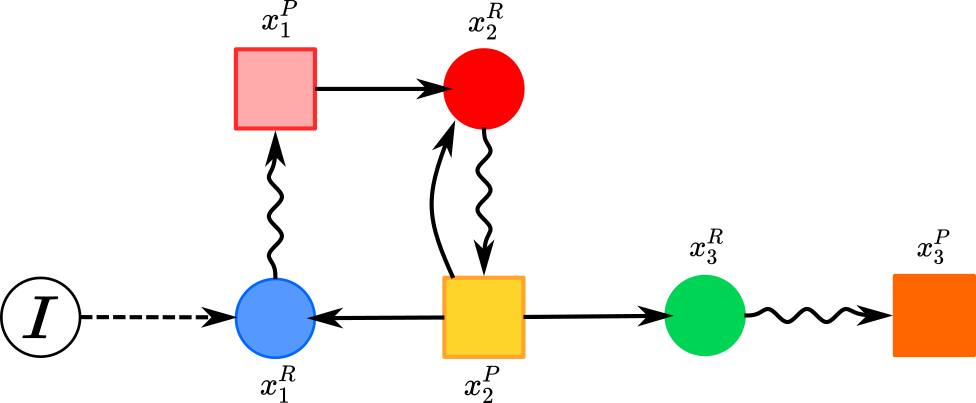
\includegraphics[scale=0.5]{figs/quotient_fibo_1.png}
    \caption{}
    \label{fig:fibo_quot}
\end{figure}


\subsubsection{Admissible vector fields}

The general possible dynamics restricted by
the topology of this network is given by the following system of 
admissible equations \cite{martin_ian_groupoids2006}:
\begin{equation}
    \begin{aligned}
        \dot{x_1}^R &= f_{x_1^R}(x_1^R, x_2^P, \mathcal{I})\\
        \dot{x_1}^P &= f_{x_1^P}(x_1^P, x_1^R)\\
        \dot{x_2}^R &= f_{x_2^R}(x_2^R, x_1^P, x_2^P)\\
        \dot{x_2}^P &= f_{x_2^P}(x_2^P, x_2^R)\\
        \dot{x_3}^R &= f_{x_3^R}(x_3^R, x_2^P)\\
        \dot{x_3}^P &= f_{x_3^P}(x_3^P, x_3^R)
    \end{aligned},
\end{equation} 
where $\vec{F} = (f_{x_1^R}, f_{x_1^P}, f_{x_2^R}, f_{x_2^P}, 
f_{x_3^R}, f_{x_3^P})$ is 
the vector of nonlinear functions as described in 
section~\ref{sec:intro}. The Jacobian of this system is 
\begin{equation}
    J = 
    \begin{pmatrix}
        f_{x_1^R,x_1^R} & 0 & 0 & f_{x_1^R, x_2^P} & 0 & 0 \\
        f_{x_1^P,x_1^R} & f_{x_1^P,x_1^P} & 0 & 0 & 0 & 0 \\
        0 & f_{x_2^R,x_1^P} & f_{x_2^R,x_2^R} & f_{x_2^R,x_2^P} & 0 & 0 \\
        0 & 0 & f_{x_2^P,x_2^R} & f_{x_2^P,x_2^P} & 0 & 0 \\
        0 & 0 & 0 & f_{x_3^R,x_2^P} & f_{x_3^R,x_3^R} & 0 \\
        0 & 0 & 0 & 0 & f_{x_3^P,x_3^R} & f_{x_3^P,x_3^P} \\
    \end{pmatrix},
\end{equation} 
where the condition for stability is defined over $f_{x_3^R,x_3^R}$
and $f_{x_3^P,x_3^P}$ and the eigenvalues of the $4 \times 4$ 
block matrix defined by the first rows and columns of the Jacobian. 
Moreover, the homeostasis matrix is given by
\begin{equation}
    H = 
    \begin{pmatrix}
        f_{x_1^P,x_1^R} & f_{x_1^P,x_1^P} & 0 & 0 & 0 \\
        0 & f_{x_2^R,x_1^P} & f_{x_2^R,x_2^R} & f_{x_2^R,x_2^P} & 0 \\
        0 & 0 & f_{x_2^P,x_2^R} & f_{x_2^P,x_2^P} & 0 \\
        0 & 0 & 0 & f_{x_3^R,x_2^P} & f_{x_3^R,x_3^R} \\
        0 & 0 & 0 & 0 & f_{x_3^P,x_3^R} \\
    \end{pmatrix}.
\end{equation} 

\subsubsection{Combinations}

Considering the $| \phi_2, \ell \rangle$ fiber circuits observed in 
the \textit{E. Coli} genetic regulatory network, we have only 
one possibility, which is the case where all regulations within 
the fiber and the external loop are negative. For this possibility 
there are four possible combinations of regulation considering 
the regulations to the external node $x_3^R$ of the mRNA/Protein 
network representation. Although we show all these possibilities 
in Fig.~\ref{fig:dd} we consider in the following section only 
the case where all regulations are negative, such that we can 
observe the general form of the infinitesimal homeostasis condition 
in the quotient of the fibonacci network.

\subsubsection{Special equations and infinitesimal homeostasis}

Considering the case where all regulations are negative, we have 
the following form for the special equations
\begin{equation}
    \begin{aligned}
        \dot{x_1}^R &= -\delta_1 x_1^R + \gamma_1 S(x_2^P) + \mathcal{I}\\
        \dot{x_1}^P &= -\alpha_1 x_1^P + \beta_1 x_1^R\\
        \dot{x_2}^R &= -\delta_2 x_2^R + \gamma_2 T(x_1^P + x_2^P)\\
        \dot{x_2}^P &= -\alpha_2 x_2^P + \beta_2 x_2^R\\
        \dot{x_3}^R &= -\delta_3 x_3^R + \gamma_3 S(x_2^P)\\
        \dot{x_3}^P &= -\alpha_3 x_3^P + \beta_3 x_3^R
    \end{aligned},
\end{equation}
where $S(x)$ is a Hill function of one variable and $T(x+y)$ is the Hill 
function over two variables.  Moreover, since the matrix $H$ is triangular, we have that 
the infinitesimal homeostasis condition is simply the multiplication
of the factors in the principal diagonal of $H$. Therefore, 
for the special equations above, we have that 
\begin{equation}
    det(H)(I_0) = \beta_1 T'(x_1^P(I_0) + x_2^P(I_0))\beta_2 S'(x_2^P(I_0)) \beta_3 
    = 0,
\end{equation}
which again provides trivial conditions for the occurrence of
infinitesimal homeostasis point, since $\beta_i \neq 0$ and the derivative
of the Hill function only goes zero for a null argument or 
asymptotically for $x_1^P + x_2^P$ (or only $x_2^P$) large enough
in the saturation regime. Changing the type of the regulations will 
only change the sign of the derivative of the Hill functions in 
the determinant of $H$. 